\documentclass[a4paper, 12pt]{article}
\usepackage{graphicx}
\usepackage[czech]{babel}
\usepackage[utf8]{inputenc}
\usepackage[T1]{fontenc}
\usepackage{amsmath}
\usepackage{amssymb}
\usepackage{pdfpages}
\usepackage{mathrsfs}
\usepackage{siunitx}
\usepackage{xcolor}
\usepackage{titlesec}
\usepackage{wrapfig}

\setcounter{secnumdepth}{4}

\titleformat{\paragraph}
{\normalfont\normalsize\bfseries}{\theparagraph}{1em}{}
\titlespacing*{\paragraph}
{0pt}{3.25ex plus 1ex minus .2ex}{1.5ex plus .2ex}

\sisetup{%
     output-decimal-marker = {.},
     inter-unit-product = \ensuremath{{}\cdot{}}
        }
        
\author{A18B0474P - Jiří Švamberg}
\title{Projekt 5}
\date{\today}

\setlength{\hoffset}{-1.8cm} 
\setlength{\voffset}{-2cm}
\setlength{\textheight}{24.0cm} 
\setlength{\textwidth}{17cm}

\begin{document}
	\begin{titlepage}
		\maketitle
		\begin{figure}
			\centering
			
\includegraphics{Obrazky/FAV-logo.pdf}
			
\includegraphics{Obrazky/zcu-logo.pdf}
			
\includegraphics[scale=0.3]{Obrazky/KKY_logo_cz.pdf}
		\end{figure}
		\thispagestyle{empty}
		\newpage
	\end{titlepage}

	\tableofcontents
	\newpage
	\section{Zadání}
		\begin{enumerate}
			\item Navrhněte zjednodušený model soustavy kvadrotorová helikoptéra - břemeno\\
			\item Pro zjednodušený model navrhněte regulátor\\
			\item Implementujte regulátor do zjednodušeného modelu\\
		\end{enumerate}
		\clearpage
	\section{Návrh zjednodušeného modelu}
		Zjednodušený model budeme navrhovat ve 2D jako kyvadlo zavěšené na vozíku.
		\begin{wrapfigure}{r}{0pt}
			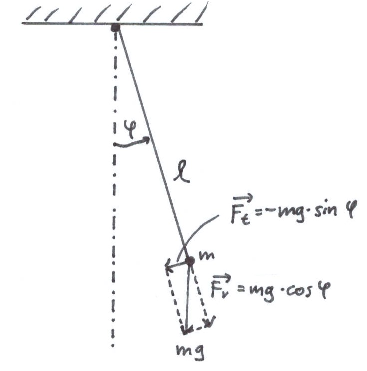
\includegraphics[scale=0.75]{Obrazky/Kyvadlo.pdf}
			\caption{Schéma jednoduchého kyvadla}
			\label{schema kyvadla}
		%\end{wrapfigure}
		%\begin{wrapfigure}{r}{0pt}
			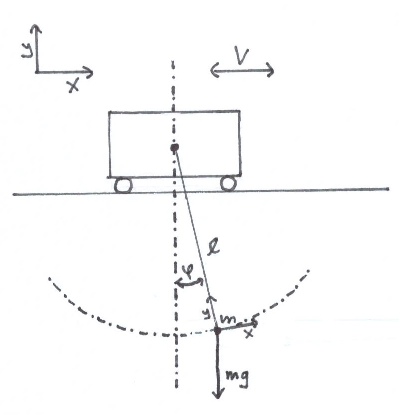
\includegraphics[scale=0.75]{Obrazky/Vozik-kyvadlo.pdf}
			\caption{Schéma soustavy vozík-kyvadlo}
			\label{schema vozik-kyvadlo}
		\end{wrapfigure}
		Pro potřeby návrhu tohoto modelu budeme uvažovat lano závěsu jako dokonale nepružné, o stálé délce $l$ a nulové hmotnosti $m_l = \SI{0}{\kilogram}$. Úhel vychýlení závěsu od osy vozíku označíme jako $\varphi$. Jako těleso si představíme bezrozměrný hmotný bod o hmotnosti $m$.\\
		Pro jednoduché kyvadlo připevněné k nepohybujícímu se tělesu o kinetické energii $T = \frac{1}{2}mv^2$ a potenciální energii $V = -mgl\cos\varphi$ (obr. \ref{schema kyvadla}) platí pohybová rovnice:
		\begin{align*}
			\ddot{\varphi}+\frac{g}{l}\sin\varphi=0
		\end{align*}
		Po zavěšení jednoduchého kyvadla na vozík(obr. \ref{schema vozik-kyvadlo}) budeme muset ještě do modelu přidat dynamiku vozíku o hmotnosti $M$. Na ten může působit síla ve směru osy x. Pro hmotný bod, zavěšený na laně budeme muset spočítat souřadnice $\left[u, v\right]$, jelikož při pohybu vozíku se nepohybuje po jasné trajektorii (kružnice, přímka):
		\begin{align*}
			u &= x + l\sin\varphi \rightarrow \dot{u} = \dot{x}+l\dot{\varphi}\cos\varphi\\
			v &= l\cos\varphi \rightarrow \dot{v} = -l\dot{\varphi}\sin\varphi
		\end{align*} 
		K odvození modelu využijeme Lagrangeovu metodu.\\
		Potenciální energii $V$ budeme uvažovat stejnou, jako u jednoduchého kyvadla.
		\begin{align*}
			V = -mgl\cos{\varphi}
		\end{align*}
		Jako základ pro vzorec kinetické energie použijeme vzorec kinetické energie obyčejného matematického kyvadla $T = \frac{1}{2}mv^2$. Musíme ale uvažovat rychlost ve směru všech souřadnic ($x$, $u$, $v$).
		\begin{align*}
			T &= \frac{1}{2}M\dot{x}^2+\frac{1}{2}m\dot{u}^2+\frac{1}{2}m\dot{v}^2
		\end{align*}
		Po dosazení souřadnic pro hmotný bod zavěšený na laně dostaneme kinetickou energii ve tvaru:
		\begin{align*}
			T &= \frac{1}{2}M\dot{x}^2+\frac{1}{2}m\left(\dot{x}+l\dot{\varphi}\cos\varphi\right)^2+\frac{1}{2}m\left(-l\dot{\varphi}\sin\varphi\right)^2
		\end{align*}
		Zjistíme si Lagrangián $L = T - V$:
		\begin{align*}
			L = \frac{1}{2}M\dot{x}+\frac{1}{2}m\left(\dot{x}+l\dot{\varphi}\cos\varphi\right)^2+\frac{1}{2}m\left(l\dot{\varphi}\sin\varphi\right)^2+mgl\cos\varphi
		\end{align*}
		, který nyní budeme parciálně derivovat.
		\begin{align*}
			\frac{\partial L}{\partial\dot{x}} &= M\dot{x}+m\dot{x}+ml\dot{\varphi}\cos\varphi\\
			\frac{\partial L}{\partial x} &= 0\\
			\frac{\partial L}{\partial \dot{\varphi}} &= m\dot{x}l\cos\varphi - ml^2\dot{\varphi}\\
			\frac{\partial L}{\partial \varphi} &= -m\dot{x}l\dot{\varphi}\sin\varphi-l^2\dot{\varphi}^2\cos\varphi\sin\varphi+ml^2\dot{\varphi}^2\sin\varphi\cos\varphi-mgl\sin\varphi
		\end{align*}
		Vztahy pro hledané dvě rovnice vypadají následovně:
		\begin{align*}
			\frac{\mathrm{d}}{\mathrm{d}t}\left(\frac{\partial L}{\partial \dot{x}}\right)-\frac{\partial L}{\partial x} = f\\
			\frac{\mathrm{d}}{\mathrm{d}t}\left(\frac{\partial L}{\partial \dot{\varphi}}\right)-\frac{\partial L}{\partial \varphi} = 0
		\end{align*}
		, kde f je síla působící na vozík. Nyní můžeme dopočítat dvě rovnice modelu vozík-kyvadlo.
		\begin{align*}
			\left(M+m\right)\ddot{x}+ml\ddot{\varphi}\cos\varphi-ml\dot{\varphi}^2\sin\varphi = f\\
			\ddot{x}\cos\varphi+g\sin\varphi-l\ddot{\varphi} = 0
		\end{align*}
			
\end{document}